\documentclass[a4paper,12pt]{report}
\def\magyarOptions{defaults=hu-min}

\usepackage[magyar]{babel}
\usepackage{t1enc}
\usepackage{indentfirst}
\usepackage[utf8]{inputenc}
\usepackage{url}
\usepackage{times}
\usepackage{subfigure}
\usepackage{amsmath}
\usepackage{amssymb}
\usepackage{amsthm}
\usepackage{verbatim}
\usepackage{fancyhdr}
\usepackage{graphicx}
\usepackage{psfrag}
\usepackage{setspace}
\usepackage[numbers]{natbib}
\usepackage{color}
\usepackage{xcolor}
\usepackage{listings}
\usepackage{todonotes}
\usepackage{rotating}
\usepackage{siunitx}

\bibliographystyle{abbrvnat}

\hoffset -0.85in
\voffset -1.5in
\oddsidemargin 30mm
\evensidemargin 20mm
\textwidth 150mm
\topmargin 30mm
\textheight 237mm
\onehalfspacing

\definecolor{codegreen}{rgb}{0,0.6,0}
\definecolor{codegray}{rgb}{0.5,0.5,0.5}
\definecolor{codepurple}{rgb}{0.58,0,0.82}
\definecolor{backcolour}{rgb}{0.95,0.95,0.92}
 
\lstdefinestyle{mystyle}{
    backgroundcolor=\color{backcolour},   
    commentstyle=\color{codegreen},
    keywordstyle=\color{magenta},
    numberstyle=\tiny\color{codegray},
    stringstyle=\color{codepurple},
    basicstyle=\footnotesize,
    breakatwhitespace=false,         
    breaklines=true,                 
    captionpos=b,                    
    keepspaces=true,                 
    numbers=left,                    
    numbersep=5pt,                  
    showspaces=false,                
    showstringspaces=false,
    showtabs=false,                  
    tabsize=2
}
\renewcommand{\lstlistingname}{Forráskód}
\lstset{style=mystyle}

%%%%%%%%%%%%%%%%%%%%%%%%%%%%%%%%%%%%%%%%%%%%%%%%%%%%%%

\begin{document}

\begin{singlespace}

\fancypagestyle{plain}{
\fancyhf{}
\fancyfoot[R]{\thepage}
\renewcommand{\headrulewidth}{0pt}
}

\pagestyle{fancy}
\fancyhf{}
\fancyhead[R]{Valós idejű rendőr-ágens irányító a Robocar World Championshiphez}
\fancyfoot[R]{\thepage}

\thispagestyle{empty}

\begin{center}
\vspace*{1cm}
{\Large\bf Debreceni Egyetem}
\vspace{0.2cm}

{\Large\bf Informatikai Kar}
\vspace{0.2cm}

{Információ Technológia Tanszék}
\vspace*{2.8cm}

{\LARGE\bf Valós idejű rendőr-ágens irányító a Robocar World Championshiphez}
\vspace*{6cm}


{\large
\begin{tabular}{c@{\hspace{3cm}}c}
\emph{Témavezető:}      &       \emph{Készítette:}\\
\bf{dr. Bátfai Norbert} &       \bf{Balkus Gergő Máté}\\
egyetemi adjunktus      &        programtervező informatikus hallgató\\
\end{tabular}
}

\vspace*{1cm}

\begin{center}
{\large
\begin{tabular}{c}
\vspace{5mm}
{A dolgozat benyújtásához hozzájárulok.}\\

\makebox[3in]{\hrulefill}  \\
dr. Bátfai Norbert\\
\end{tabular}
}
\end{center}

\end{center}

\vspace{25mm}
\begin{center}
{\Large
Debrecen
\\
\vspace{2mm}
2016
}
\end{center}

\tableofcontents

\end{singlespace}
%%%%%%%%%%%%%%%%%%%%%%%%%%%%%%%%%%%%%%%%%%%%%%%%%%%%%%%%%%%%%%%%%%%%%%%%%%%%%%%%%%%%%%%%%%%%%%%%%%%%%%%%%%%%%%%%%%%%%%%%%%%

\chapter{Bevezetés}

\begin{figure}[ht]
\centerline{
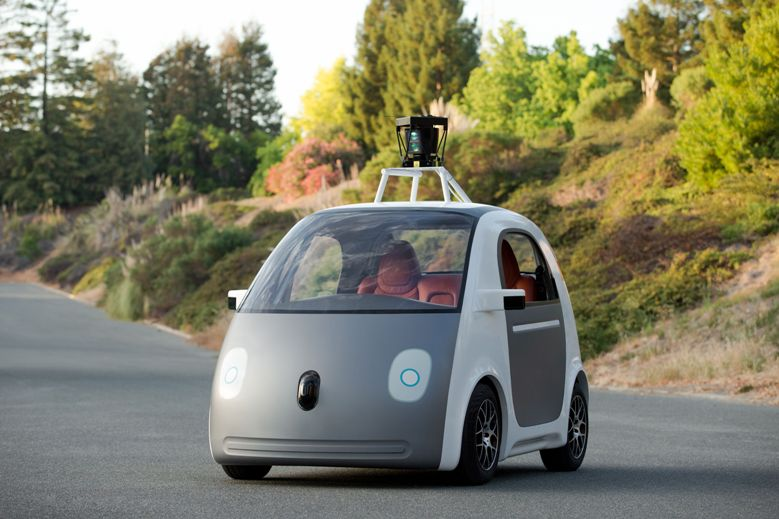
\includegraphics[width=6in]{img/googleauto}}
\caption{A Google által fejlesztett robotautó. Forrás: \cite{googlecarimage}.}
\label{googleauto}
\end{figure}

A közelmúltban nagy mértékű fejlődést vehettünk észre az autógyártásban, különösképp a magukat irányítani tudó autók kapcsán. Több és több autók gyártásával foglalkozó cég fejleszt robotautót. Ilyen például ezen a területen az elsőként megjelenő Google, melynek a robotautóját a \ref{googleauto}. képen láthatjuk. Ezek a szokások dinamikus fejlődést mutatnak. A 2000-es évektől kezdve az autók elektronikus eszközei jelentős mértékben arról szóltak, hogy azok segítették a vezetőt különböző módokon. Ilyen eszközök például a tolató radarok, illetve a gyalogosfigyelő rendszerek is. 

\vspace{2mm}
Az elkövetkező éveket azonban várhatóan az autonóm autók nagy mértékű megjelenése és elterjedése váltja fel. Ezek az autók mellett nemrég láthattuk a Tesla új modelljének a bemutatóját is, mely ugyancsak erősíti a feltevést, miszerint az elektromos hajtású, illetve az úgynevezett ``hibrid'' hajtású kocsik előtt áll a jövő. Elektromos hajtású kocsikat manapság is láthatunk már az utcákon. Ezeket könnyen felismerhetjük a zöld hátterű rendszámtáblájukról.

\vspace{2mm}
A Drive.ai a 13. cég akik jogosítványt kaptak az autonóm kocsik teszteléséhez Kalifornia publikus utcáin. A cég az autonóm autók továbbfejlesztésén dolgozik úgy, hogy a mély-tanulást (deep-learning) alkalmazza robotautókra. Ez azért kiemelkedően fontos, mert az autonóm kocsik fejlesztésében a kemény rész a szélsőséges esetek (edge cases) megoldása. Ilyen esetek lehetnek például a havazás, vagy az eső is. Jelenleg az autonóm kocsik fejlesztői különböző szabályokat programoztak be ezekre az esetekre, azonban a mély-tanulás megközelítésével a robotautó megtanulja hogy reagáljon ezekre az esetekre azáltal, hogy a kapott adat teljes egészét próbálja megérteni, és a már megtanult adat alapján reagál rá. \cite{driveai}.

\vspace{2mm}
A fent említettek alapján tisztán látszik, hogy az autóipar szemléletváltás előtt áll. A nem újrahasznosítható energiaforrásokon alapuló motorokat és a vezetői élményt kezdi lassan felváltani a hosszabb távon fenntartható, újrahasznosítható energiaforrást használó motorokkal hajtott autonóm gépkocsik, mellyel az utazáshoz a pihentető időtöltés vízióját próbálják hozzárendelni.

\begin{figure}[ht]
\centerline{
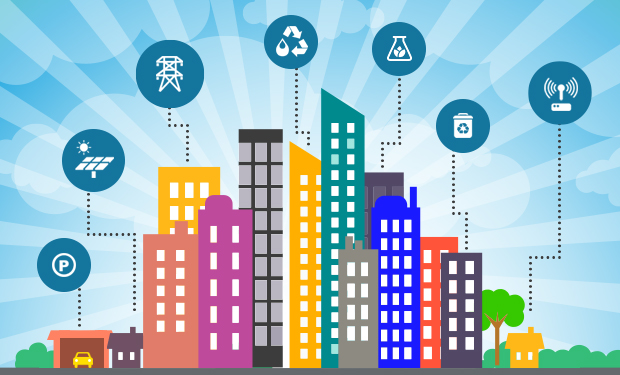
\includegraphics[width=6in]{img/smartcitylogo}}
\caption{Egy elképzelt okos város vektorgrafikus ábrázolása. Forrás: \cite{smartcitylogo}.}
\label{smartcitylogo}
\end{figure}

\vspace{2mm}
2050-re a világ lakosságának 70\%-a valószínűleg városokban fog élni \cite{unpopulation}. Ez a gyors városiasodás új kihívásokat állít fel a város infrastruktúrája felé. Több kérdés is felmerül ilyenkor. Hogyan tudunk biztonságosan ``irányítani'' egy ilyen nagy méretű népességet? Mely szolgáltatásokkal lássa el a városi ügyintézés azért, hogy fenntartható legyen a város? 

\vspace{2mm}
Ezeket a kérdéseket is megválaszolja az Okos városok kutatási területe, mely eredményei egyre inkább láthatóak a mindennapi életben is. Talán az egyik legfontosabb kérdés ez ügyben a városi közlekedés. Ahogy nő a népesség, úgy nő azok az emberek (és kocsik) száma akik a város infrastruktúráját, illetve úthálózatát használják. Hogyan tud segíteni a városi management, hogy az ott élők a lehető leghatékonyabban tudjanak közlekedni? Ezt a kérdést válaszolja meg a smart traffic management.

\vspace{2mm}
Az Smart City Research and Development terület láthatóan fontos szerepet fog kapni az elkövetkezendő 10-20 évben. Előrejelzések azt mutatják, hogy 2023-ra több mint 170 milliárd USD beruházás valósul meg a világon \cite{navigant}. Az informatikai fejlesztések ezen a téren már egyre jobban beférkőztek a hétköznapokba is, mint például az iCity \cite{icity}, a FI\-Ware \cite{fiware}, vagy a \cite{vital}. Ezeken túl egyre többen kísérleteznek azzal, hogy a város embereinek a mindennapjait hatékonyabbá és biztonságosabbá varázsolja (\cite{myneighbourhood}, \cite{smartsantander}).

\vspace{2mm}
Sok tanulmány foglalkozik még azzal, hogy hogyan lehetne egy városnak az ``okosságát'' megmérni (\cite{de2014smart}, \cite{carli2013measuring}). A városok ``okosságáról'' még egy sorrendet is készítettek \cite{giffinger2007smart}. Az okos városokban a vészhelyzetek megoldása is fontos szerepet kap \cite{du2012research}.

\chapter{A Robocar World Championship (OOCWC)}
\label{oocwc}

\section{Ismerkedés az OOCWC rendszerrel}

Az OOCWC rendszer célja, hogy az autonóm autók és az okos városok közötti összefüggéseket vizsgálja, kutatási valamint oktatási célokat is szolgál. A rendszer felépítését a \ref{basedesign}. ábra szemlélteti.

\begin{figure}[ht]
\centerline{
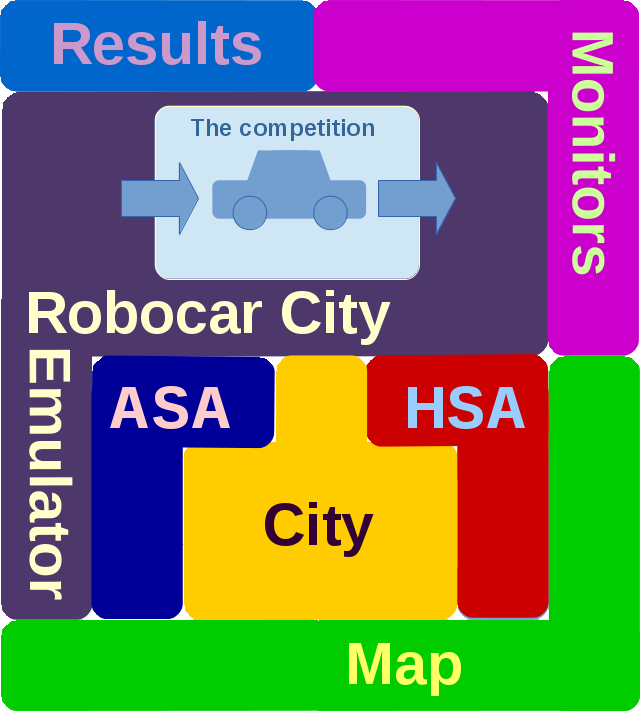
\includegraphics[width=3.7in]{img/tetris_plan}}
\caption{Az OOCWC rendszer tetris terve. Forrás: \cite{oocwcrepo}.}
\label{basedesign}
\end{figure}

Ez alapján a rendszer egyes elemei:

\begin{itemize}
\item Map -- a szimuláció egy adott térképen értelmezett,
\item City -- a szimuláció működési egysége,
\item The competition -- a verseny célja / maga a verseny,
\item ASA -- automatikus adatgyűjtő rendszer,
\item HSA -- kézi adatgyűjtő rendszer,
\item Robocar City Emulator -- forgalom emuláció,
\item Results -- a verseny eredményei, illetve kísérletek eredményei,
\item Monitors -- megjelenítők, vizualizáció.
\end{itemize}

A rendszer egyrészt egy kutatási platformot kínál forgalomelemzésre, szimulációkra, másrészt pedig egy érdekes versenyzési platformot nyújt.

\vspace{2mm}
A verseny célja az, hogy találjuk meg a lehető legjobb forgalomirányító algoritmust. Az OOCWC már több sikeres versenyen is túl van a Debreceni Egyetem Informatikai Karán \cite{competitions}. Gyakori, hogy egy kutatás által létrejött rendszerre versenyt szerveznek a felhasználók körében. Erre egy jó példa az mesterséges intelligencia (AI - Artificial Intelligence) területén a RoboCup \cite{robocup}.

\vspace{2mm}
Fontos megemlíteni, hogy a Robocar World Cup kiválóan alkalmazkodik a különböző esetekre. Az oktatás és kutatások támogatására került kifejlesztésre a ``Police Edition'' (egy pillanatkép ebből a változatból a \ref{police}. ábrán látható). A cél, hogy rendőr-ágensekkel, melyeket a felhasználó által megírt irányító algoritmus vezérel, minél több gengszter-ágenst kapjunk el.

\vspace{2mm}
A rendszer jelenleg háromféle forgalmi egységet különböztet meg, routine cars, smart cars és guided cars. A szimuláció kezdőállapota a routine cars és smart cars elhelyezése a térképen a gyűjtött adatok alapján.

\vspace{2mm}
A rendszer ``Police Edition'' változatából készíthetnek egy saját fork-ot a hallgatók és az érdeklődő kutatók. A játék célja, hogy a rendőr ágensekkel minél több gengszter ágenst kapjunk el. A bemutatott projekt (\ref{theapp}. fejezet) is egy ilyen forknak tekinthető.

\vspace{2mm}
A rendszerről további információk olvashatóak a \cite{infocomjournal} közleményben.

\section{A rendszer elindítása}
\label{howtostart}

A továbbiakban tételezzük fel hogy a projektben a szükséges forráskódokat már lefordítottuk, így binárisan elérhetőek, továbbá jelenleg az ``rcemu'' mappában vagyunk, és a szülőmappában elérhető . Ehhez segítséget az OOCWC eredeti tárolóján \cite{oocwcrepo} találhatunk.

\vspace{2mm}
Elsőnek az okos városunkat kell elindítani. Ezt a \ref{startsmartcity}. forráskódban látható Bash parancs futtatásával  tehetjük meg.

\lstinputlisting[language=bash, caption=A SmartCity elindítása, label=startsmartcity]{src/smartcity.sh}

Itt a kapcsolók a következő beállításokat jelentik:

\begin{itemize}
\item osm -- Az OpenStreetMap térkép elérési útvonala.
\item city -- A szimulált város neve.
\item shm -- Az osztott memória elérési neve.
\end{itemize}

Amennyiben a SmartCity kimenetén megjelenik hogy ``Ready'', úgy folytathatjuk a következő lépéssel, a szimulációs szerver elindításával, melynek a parancsát a \ref{starttraffic}. forráskódban láthatjuk.

\lstinputlisting[language=bash, caption=A szimulációs szerver elindítása, label=starttraffic]{src/traffic.sh}

A beállítási kapcsolók jelentése a következő:

\begin{itemize}
\item port -- A szervernek a portja, amelyen a szerver üzemel.
\item shm -- Az osztott memória neve.
\end{itemize}

\section{A rendszer működése}

\subsection{Az adat áramlása}
\label{dataflow}

\begin{figure}[ht]
\centerline{
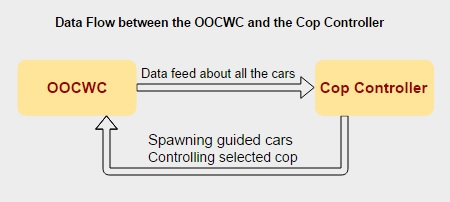
\includegraphics[width=4.5in]{img/dataflow}}
\caption{Az adat áramlása az OOCWC rendszer (\ref{oocwc}. fejezet) és az alkalmazás (\ref{theapp}. fejezet) között.}
\label{dataflowpicture}
\end{figure}

Ahogy a \ref{dataflowpicture}. ábrán látható, ahogy folyik a szimuláció a szerveren, úgy minden egyes lépésenként a szerver elküldi az aktuális állást az alkalmazásnak. Ezt a Cop Controller feldolgozza, ezáltal valós idejű képet adva a jelenleg állásról.

\vspace{2mm}
Az alkalmazás oldaláról több funkciót is lehet használni. Ezekről többet a \ref{functions}. fejezetben olvashatsz. Ezek a funkciók azonnal feldolgozásra kerülnek a szerveren, így a változás azonnal látható lesz.

\section{Szükséges módosítások a projekt számára}
\label{changes}

\subsection{Az eredeti irányítás}
\label{originalrouting}

Eredetileg a rendőr-ágensek is C++ nyelven (\ref{cplusplus}. fejezet) lettek megvalósítva, ezáltal hozzáférnek az OOCWC osztott memóriájához (shared memory), amiben több adat közt megtalálható az OSM \citep{osm} (\ref{osm}. fejezet) térképből felépített irányított gráf (BGL (Boost Graph Library)) (\ref{boost}. fejezet). Ezt a gráfot és a Boost, gráfokra implementált, kereső algoritmusait felhasználva a rendőr-ágens képes létrehozni a szimulációs szerver által értelmezhető útkereső (routing) parancsot, mellyel a szerver a kapott parancs alapján mozgatja a megfelelő rendőr-ágenst. 

\vspace{2mm}
Az eredeti parancs a következőképp néz ki: 
\begin{lstlisting}
<route [a csomopontok szama: N] [rendor-agens ID] [N darab csomopont]>
\end{lstlisting}

Ez a parancs a \ref{originalroutingsrc}. forráskódrészleten látható módon lesz feldolgozva.

\lstinputlisting[language=C++, caption=Az eredeti routing forráskód részlete, label=originalroutingsrc]{src/originalroutingcmd.cpp}

\subsection{Az új irányítás}
\label{newrouting}

Ahhoz hogy az eredeti irányításhoz hasonló mozgatást érjünk el a kívánt rendőr-ágensen, egy olyan programozási nyelvvel amelynek nincs hozzáférése az OOCWC által felépített osztott memóriához, egy új parancs bevezetésére volt szükség, amely helyettesíti az eredeti útkereső parancsot, a valódi routingot (az út megtalálását kettő csomópont között) pedig a szerverre kellett bízni.

\vspace{2mm}
Ennek a változtatásnak a bevezetésével úgy vélem hogy egy új lehetőség nyílik meg az OOCWC rendszer számára, mégpedig hogy több programozási nyelv segítségével is meg lehessen jeleníteni az aktuális állapotot, illetve lehessen általuk irányítani a rendőr-ágenseket. (I'm looking at you, Python)

\vspace{2mm}
Az új parancs a következőképpen néz ki:
\begin{lstlisting}
<inner_route [rendor-agens ID] [A cel csomopont]>
\end{lstlisting}

TODO az új parancs szintaxisának bemutatása

TODO forráskód az új routingról

\newpage
\chapter{Felhasznált technológiák}
\label{technologies}

\section{Java}
\label{java}

\begin{figure}[ht]
\centerline{

\includegraphics[width=1.1in]{img/javalogo}}
\caption{A Java hivatalos logója.}
\label{javalogo}
\end{figure}

A Java programozási nyelv az alapja a hálózati alkalmazások nagy részének, és világkörű szabvány a beágyazott mobil alkalmazások, játékok, webes tartalmak, és a vállalati szoftverek számára. Több mint 9 millió fejlesztővel világszerte a háta mögött, a Java az egyik leghasználtabb és legelterjedtebb programozási nyelv. 

\vspace{2mm}
Néhány érdekes tény a Java nyelvről:

\begin{itemize}
\item 97\%-a a vállalati számítógépeknek futtat Javát.
\item 89\%-a az asztali komputereknek az Amerikai Egyesül Államokban képes Javát futtatni.
\item A fejlesztők első számú választása.
\item Az első számú fejlesztési platform.
\item 3 milliárd mobil eszközön tudnak futni Java alkalmazások.
\item 125 millió TV készülékek képesek Java alkalmazásokat futtatni.
\end{itemize}

\vspace{2mm}
A Java úgy lett kialakítva, hogy lehetővé váljon a hordozható, nagy teljesítményű alkalmazások fejlesztése a legszélesebb körű számítástechnikai platformok számára. Azáltal hogy az alkalmazások heterogén környezetekben elérhetővé válnak, a különböző vállalkozások képesek több szolgáltatást nyújtani, és megnöveli a a végfelhasználói produktivitást, kommunikációt és együttműködést -- és drasztikusan csökkennek a fenntartási költségek mind a vállalati, mind a fogyasztói alkalmazások körében. A Java felbecsülhetetlenné vált a fejlesztők számára azáltal, hogy lehetővé tette:

\begin{itemize}
\item A szoftverek megírását egy platformon, és annak futtatását virtuálisan bármely másik platformon;
\item Olyan programok létrehozását, melyek egy internetes böngészőn belül futnak, és hozzáférése van az elérhető internetes szolgáltatásokhoz;
\item A Javában írt alkalmazások, illetve szolgáltatások, összeillesztését annak érdekében, hogy magasan személyre szabott alkalmazásokat / szolgáltatásokat fejlesszünk \cite{aboutjava}.
\end{itemize}

\lstinputlisting[language=Java, caption=A klasszikus ``Hello World!'' Javában, label=helloworldjava]{src/helloworld.java}


\subsection{Története}
\label{javahistory}

Manapság, amikor a technológia már ennyire része a mindennapi életünknek, magától értetődőnek tartjuk, hogy bármikor és bárhol elérhetővé válnak az alkalmazások és a keresett tartalmak. A Java nyelv miatt napjainkban már elvártnak tekintjük a digitális eszközeinktől hogy több funkcióval rendelkezzenek, okosabbak és jóval szórakoztatóbbak legyenek.

\vspace{2mm}
Az 1990-es évek elején a hálózati számítás kierjesztése a mindennapi életre egy radikális elképzelésnek számított. 1991-ben egy kis csoportja a Sun mérnökeinek, akik a ``Green Team'' csapatnevet viselték, James Gosling irányításával létrehoztak egy új programozási nyelvet -- a Javát \cite{javahistory}.

\subsection{Objektumorientáltság}
\label{oo}

A Java nyelv egyik legfontosabb tulajdonsága az objektumorientáltsága, ami a nyelv felépítésére és stílusára is mutat. 

\vspace{2mm}
A C++ nyelvvel ellentétben (lásd: \ref{cplusplus}. fejezet) a Java teljesen objektum-orientált: minden egyes Java programnak szüksége van legalább egy osztály jelenlétére. Továbbá a Java eredeti nyelv-definíciója magában foglalja az ``objektum-orientált'' kifejezést.

\vspace{2mm}
Az Objektum Orientált Programozás (röviden OOP) egyik fontos alapköve az egységbezárás (encapsulation). Mikor egy objektumot létrehozunk egy objektum-orientált nyelven, el tudjuk rejteni az objektum belső működésének a komplexitását a külső világ elől, így a külső világnak csak elég csak az objektum felhasználását ``tudnia''.

\vspace{2mm}
Másik fontos alapköve az öröklődés (inheritance). Az objektumok származtatása egy szülő-objektumból (superclass) azt a célt szolgálja, hogy a gyerek-objektumok (subclass) átveszik a superclass látható tulajdonságait és metódusait, miközben a kifejezetten csak rájuk tartozó saját tulajdonságokat, illetve metódusokat is tartalmaznak.

\subsection{Platformfüggetlenség}
\label{platformfugg}

``Write once, run anywhere'' \cite{wora}.

\vspace{2mm}
Általában a lefordított kód pontosan az az instrukcióhalmaz ami szükséges a processzor számára a program ``futtatásához''. A Java esetében azonban ez az utasításhalmaz egy virtuális processzorhoz van lefordítva, melynek működnie kell bármely fizikai számítógépen.

\vspace{2mm}
A Java esetében a fizikai processzor futtatja a JVM-et (Java Virtual Machine) ami platformfüggő. Ez a virtuális gép fogja aztán futtatni a Java bájt-kódot, ami azonban már platformfüggetlen. 

\vspace{2mm}
Az egyetlen mód arra, hogy a Java bájt-kódok valóban bármely JVM-en fussanak, az a szigorú szabvány arról, hogyan működnek a Java Virtuális Gépek. Ez azt jelenti hogy bármilyen fizikai platformot használunk, a programunknak az a része, mely a JVM-mel van kapcsolatban, garantáltan csak egy módon fog működni. Mivel mindegyik JVM pontosan ugyanúgy működik, ugyanaz a kód ugyanúgy fog működni mindenhol anélkül hogy újrafordítanánk.

\vspace{2mm}
Természetesen van módja a platformfüggetlenségét megtörni egy Java programnak. Ilyen eset például amikor olyan konvenciót használunk, amely csak az egyik operációs rendszerre igaz (például feltételezzük azt, hogy a ``:'' a könyvtárakat elválasztó szimbólum).

\subsection{Swing}
\label{swing}

A Swing egy eszközkészlet a grafikus felhasználói felületek létrehozására.

\vspace{2mm}
A Swinget azzal a céllal fejlesztették, hogy egy szofisztikáltabb GUI komponenshalmazt szolgáltasson mint a korábbi Abstract Window Toolkit (AWT) \cite{awt}. A Swingnek a komponensei erőteljesebb és flexibilisebb az AWT-hez hasonlítva. A már ismert komponensekhez, mint például a Button-ök, check boxok és labelek, a Swing olyan további fejlett eszközökkel szolgál, mint a tabbed panel, scroll pane, fák, táblázatok és listák.

\vspace{2mm}
Ellentétben az Abstract Window Toolkit komponenseivel, a Swing komponensei nem platform-specifikus kódként lettek implementálva. Helyette teljesen Java nyelven írták meg, ezáltal a komponensek platform-függetlenek lettek. A ``lightweight'' kifejezéssel írjuk le az ilyen elemeket \cite{swingarticle}.

\vspace{2mm}
A Swinget a közeljövőben a JavaFX \cite{javafx} fogja felváltani.

\subsection{JXMapViewer}
\label{jxmapviewer}

A JXMapViewer \cite{jxmapv} egy nyílt forráskódú Java könyvtár, ami egy Swing (\ref{swing}. fejezet) JPanelt \cite{jpanel} szolgáltat, melynek feladata a térkép betöltése, és mutatása.

\newpage
\section{C++}
\label{cplusplus}

A C++ egy nyílt, ISO-szabványosított programozási nyelv. Eleinte ez nem így volt, és a nyelvnek nem volt hivatalos szabványa, és csak egy de-facto szabványt követve volt karbantartva, fejlesztve, azonban 1998 óta \cite{c++98} a nyelv szabványosítva van az ISO egy bizottsága által.

\vspace{2mm}
A C++ egy ``compiled'' (lefordított) nyelv. Ahhoz hogy egy C++ programot le tudjunk futtatni, elsőnek a C++ fordító segítségével platformfüggő futtatható bájt-kódra kell fordítanunk a kódunkat. Ezáltal a C++ a világ egyik leggyorsabb nyelve, ha a kódunk optimalizálva van.

A C++ nyelv egyik fő erőssége, hogy a programozótól függ hogy mely paradigmákat követi a probléma megoldása érdekében. A C++ támogatja a procedurális, generikus, illetve az objektum-orientált programozási paradigmákat, sok más paradigmát pedig szintén lehetővé téve ezáltal.

\lstinputlisting[language=C++, caption=A klasszikus ``Hello World!'' C++-ban, label=helloworldcpp]{src/helloworld.cpp}

\subsection{Története}
\label{cpphistory}

A korai '80-as években, a Bell Laboratories cégnél, egy új programozási nyelvet kezdtek el fejleszteni, ami a C nyelvet vette alapul. Ennek az új nyelvnek a fejlesztője Bjarne Stroustrup volt, aki C++-nak keresztelte el az ``új'' nyelvet. Stroustrup azt állította, hogy a C++ célja az, hogy könnyítse és kellemesebbé tegye a jó programok írását. Amikor a nyelvet tervezte, belecsempészte az OOP (objektumorientált programozás) jellemzőit anélkül hogy nagyon módosításokra lett volna szükség a C kódjában. Így a C egy részhalmaza a C++-nak, tehát bármely érvényes C program egyben érvényes C++ program is.

\vspace{2mm}
Idővel ahogy egyre jobban fejlődött a nyelv, elkerülhetetlenné vált a szabványosítás. A C++ 1991-ben indult el a szabványosítás útján, majd 1998-ban az ISO szabványosításba bekerült ``ISO/IEC 14882:1998'' néven \cite{c++98}. A következő szabványt 2003-ban fogadták el ``ISO/IEC 14882:2003'' kódnévvel \cite{c++03}. 8 éve elteltével a következő szabványt is elfogadták, amit ``ISO/IEC 14882:2011'' kódjelzéssel láttak el \cite{c++11}. A legújabb C++ szabvány a röviden C++14 névre hallgató, ``ISO/IEC 14882:2014'' kódú szabvány \cite{c++14}.

\subsection{Boost library}
\label{boost}

\begin{figure}[ht]
\centerline{

\includegraphics[width=3.6in]{img/boost}}
\caption{A Boost logója. Forrás: \cite{boostlogo}.}
\label{boostlogo}
\end{figure}

\vspace{2mm}
A Boost a C++ programozási nyelvhez ad támogatást olyan könyvtárakkal, melyek különböző területek különböző problémáit segítenek megoldani. Többek között ilyen területek a lineáris algebra, a pszeudorandom számok generálása, a több-szálasítás, a képfeldolgozás, a reguláris kifejezések, illetve a unittesztelés. 

\vspace{2mm}
Az OOCWC (\ref{oocwc}. fejezet) számára az egyik legfontosabb ilyen könyvtár a BGL (Boost Graph Library) \cite{bgl}, melynek segítségével épül fel az OpenStreetMap \cite{osm} (\ref{osm}. fejezet) térkép alapján az OOCWC irányított gráfja.

\newpage
\section{Maven}
\label{maven}

\begin{figure}[ht]
\centerline{

\includegraphics[width=4.5in]{img/mavenlogo}}
\caption{A Maven logója. Forrás: \cite{mavenlogo}.}
\label{mavenlogo}
\end{figure}

A Maven eredetileg egy kísérletként indult azzal a céllal, hogy a Jakarta Turbine projekt \cite{turbine} build folyamatait egyszerűsítsék. Több projekt volt a saját Ant \cite{ant} build fájljaival, melyek alig voltak különbözőek. A Maven célja az (volt), hogy létrehozzon egy szabványosított módszert arra, hogy:

\begin{itemize}
\item hogyan legyenek a projektek buildelve,
\item tiszta és egyértelmű leírás legyen a projekt függőségeit tekintve,
\item könnyen lehessen a projekt információit megosztani.
\end{itemize}

Az eredmény végül egy olyan eszköz lett, mellyel bármely Java alapú projektet könnyen tudjuk építeni és menedzselni. A Maven működéséhez egy \url{pom.xml} fájlt kell megadni, amely tartalmazza a projekt felépítéséhez szükséges összes információt. Ilyen információ például a menedzselt projekt függősége is, melyet miután meghatároztunk a POM (Project Object Model) fájlban, a Maven letölti a hozzá tartozó JAR fájlt, és felkerül a projekt classpath-jára, ezáltal máris használni tudjuk a projekten belül az a dependenciát.

\vspace{2mm}
Ezeket a függőségeket a Maven az általa üzemeltetett Maven Repository Center-ben \cite{mavenrepository} keresi, és tölti le. Van lehetőségünk további tárolókat hozzáadni a POM fájlunkhoz, illetve saját magunk is készíthetünk tárolókat.

\newpage
\section{Git}
\label{git}

\begin{figure}[ht]
\centerline{

\includegraphics[width=3.6in]{img/gitlogo}}
\caption{A Git logója. Forrás: \cite{gitlogo}.}
\label{gitlogo}
\end{figure}

A Git egy verziókezelő rendszer, melyet széles körben használnak a szoftverfejlesztésnél és egyéb verziókövetési feladatoknál. Ez egy elosztott forráskódkezelő rendszer, melynél nagy hangsúlyt kap a sebesség \cite{gitspeed}, az adatok integritása \cite{gitdata}, és az elosztott, nem lineáris munkafolyamatok támogatása. A Gitet eredetileg 2005-ben tervezték és fejlesztették a Linux kernel fejlesztői a kernel fejlesztésének támogatására.

\vspace{2mm}
Mint a legtöbb elosztott verziókövető rendszereknél, és ellentétben a legtöbb kliens-szerver rendszerekkel, minden egyes Git munkakönyvtár egy teljes értékű Git tároló, teljes előzménnyel, és teljes verzió-követési képességgel, ami független a hálózati hozzáféréstől, vagy a központi szervertől.

\vspace{2mm}
A Gitet elsőnek egy alacsony szintű verziókezelő rendszernek tervezték, amire aztán az emberek a saját ízlésüknek megfelelő front-endet fejleszthettek. Ilyen például a Cogito \cite{cogito}. A Git mára már egy teljes verziókezelő rendszerré nőtte ki magát, és így más programok nélkül is tudjuk használni. Bár a fejlesztést erősen befolyásolta a BitKeeper \cite{bitkeeper}, Torvalds szándékosan kerülte a hagyományos megközelítéseket, amelynek köszönhetően a Git egy egyedi struktúrával jött létre \cite{gitunique}.

\newpage
\section{OpentStreetMap (OSM)}
\label{osm}

Az OpenStreetMap egy ingyenes, a közösség által szerkesztett térkép. Célja hogy az egész világot minél részletesebben leíró ingyenes térképet szolgáltassanak a szoftverfejlesztők, illetve felhasználók számára. A térképet bárki szerkesztheti aki az oldalukra (\url{www.openstreetmap.org}) regisztrál. 

\vspace{2mm}
Az OSM létrejöttét Steve Coast-nak köszönhetjük, aki 2004-ben kezdte el a projektet azzal a céllal, hogy Angliát feltérképezze. 2006 áprilisában lett létrehozva az OpenStreetMap Egyesület azzal a céllal, hogy segítse a térinformatikai adatok növekedését, fejlesztését, és forgalmazását a felhasználók körében.

\vspace{2mm}
Az önkéntesek egy Java (\ref{java}. fejezet) alapú appleten keresztül tudtak módosításokat felvinni a térképre, vagy valamely offline szerkesztő szoftver használatával. A mai napig az egyik legjobban használt ilyen program a JOSM \cite{josm}.

\vspace{2mm}
2006 decemberében a Yahoo megengedte, hogy az OpenStreetMap felhasználja a légi felvételeit, ezáltal olyan helyeket is sikerült az OSM-nek ledokumentálnia, melyekhez eddig nem tudtak hozzáférni. Fél évvel később kiadták a Potlatch \cite{potlatch} térképszerkesztőt, ezáltal segítve a robbanásszerűen növekedő felhasználóbázis integrációját. Egy példát a Potlatch térképszerkesztő 2006-os verziójára a \ref{oldworcester}. ábrán láthatunk.

\newpage
Az állandó térképszerkesztő szoftverek fejlesztéseinek köszönhetően 2009-től kezdve az OSM egyre jobban elterjedt, a felhasználó- és szerkesztőbázisa pedig exponenciálisan növekedett (lásd: \ref{osmusers}. ábra).

\begin{figure}[ht]
\centerline{
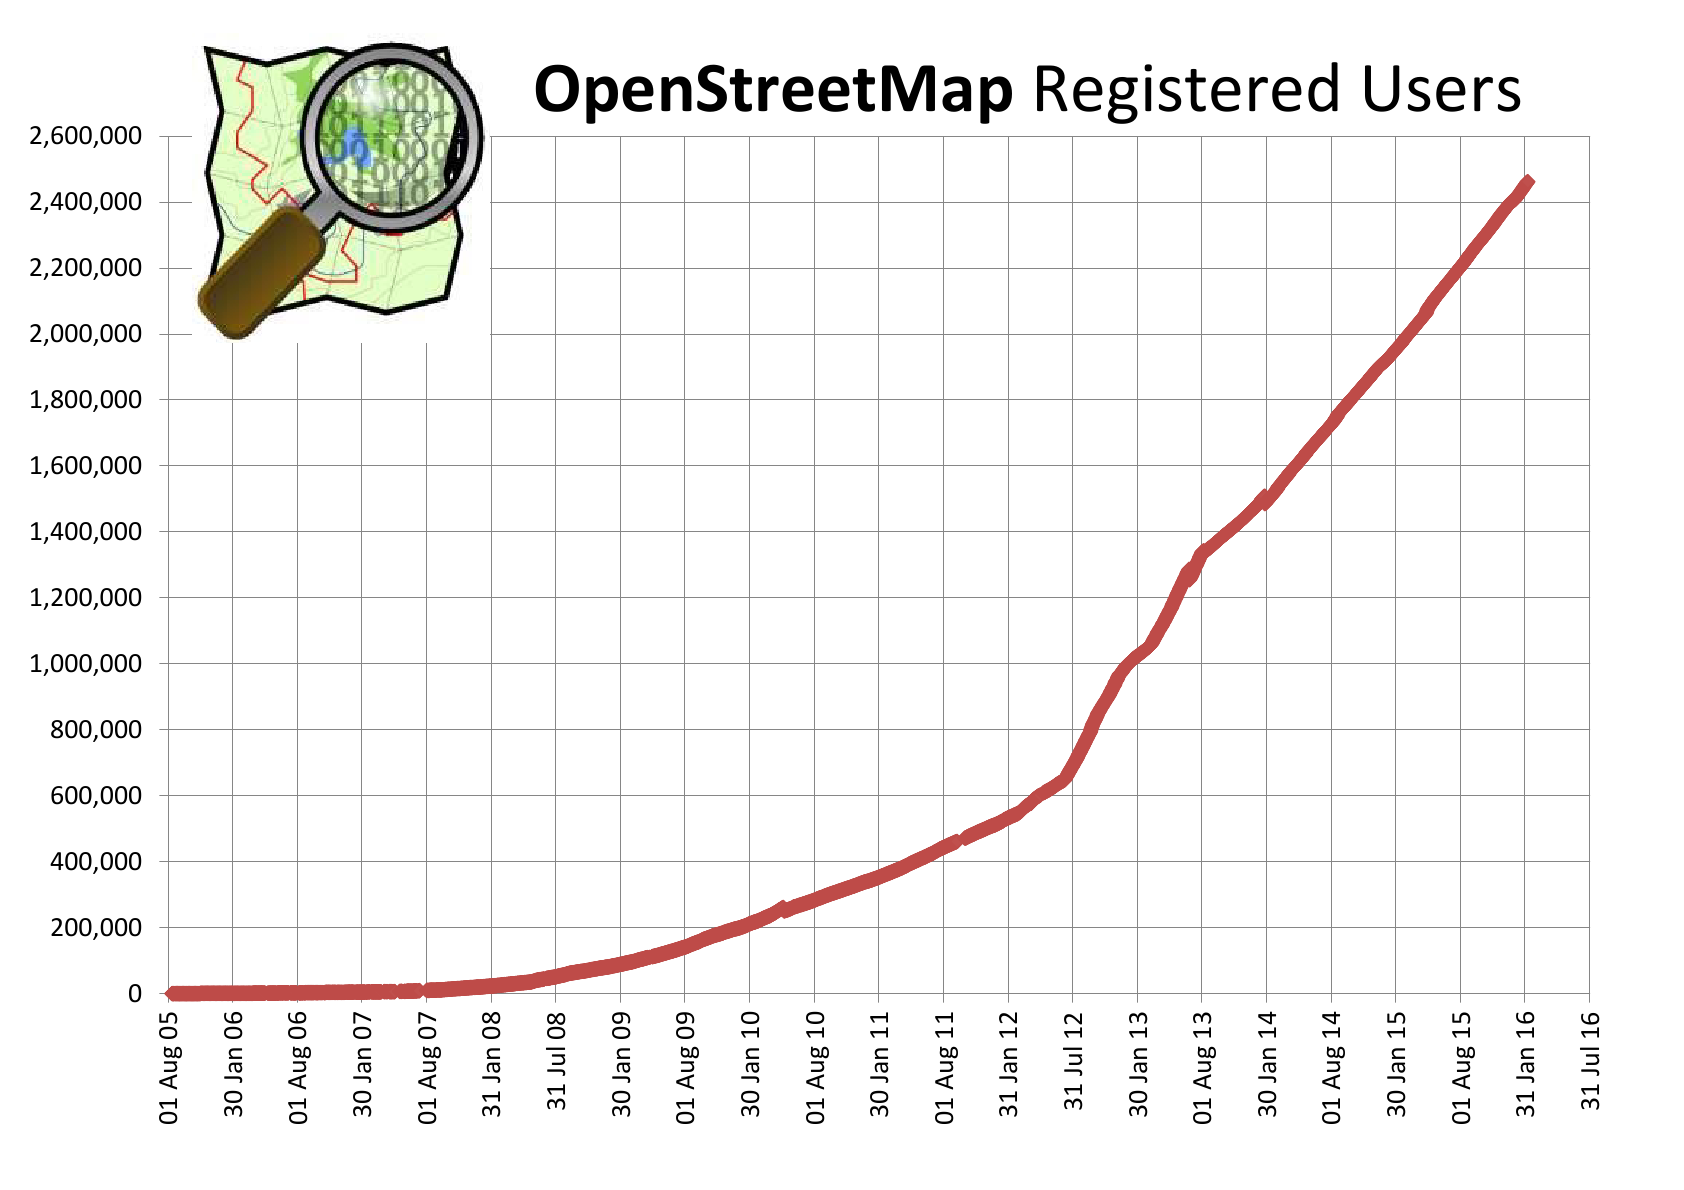
\includegraphics[width=5.5in]{img/osmusers}}
\caption{Az OpenStreetMap regisztrált felhasználóinak száma. Forrás: \cite{osmhistory}.}
\label{osmusers}
\end{figure}

A mai napra már annyira megbízható térképpé nőtte ki magát az OpenStreetMap -- hála az egyre több és több önkéntes szerkesztőnek -- hogy több nagyobb (mobil)alkalmazás is az OSM-re alapul. Ilyen például, egy a sok közül, a Maps.me \cite{mapsme} mobilalkalmazás.

\begin{figure}[ht]
\centering
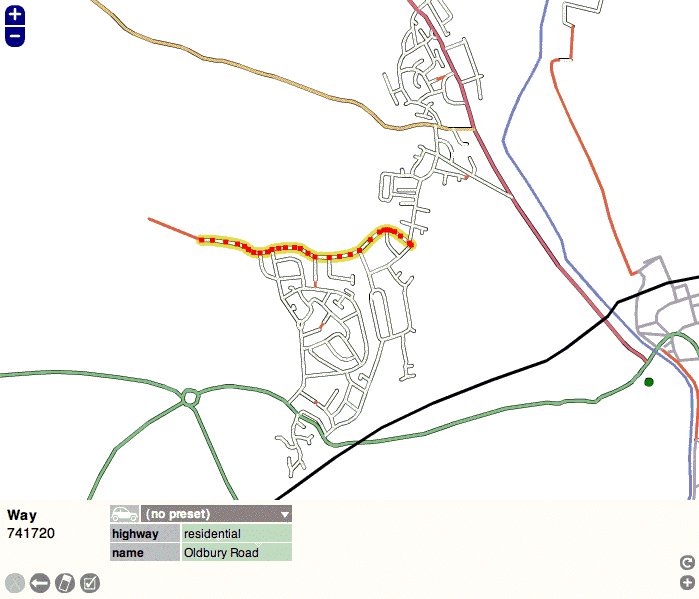
\includegraphics[width=5in]{img/oldworcester}
\caption{A Potlatch-ben szerkesztett Worcester térképe 2006-ban. Forrás: \cite{osmhistory}.}
\label{oldworcester}
\end{figure}

\begin{figure}
\centering
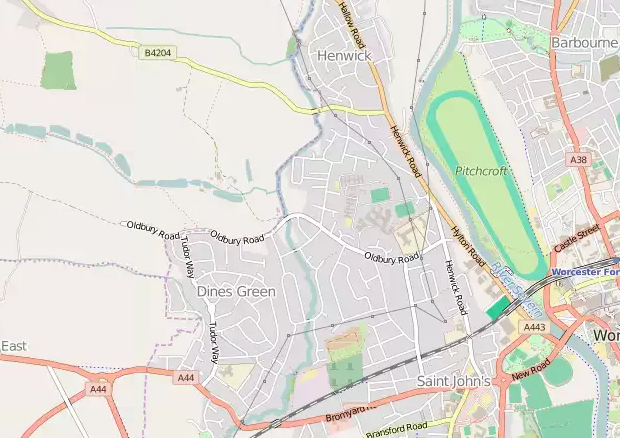
\includegraphics[width=5in]{img/newworcester}
\caption{Worcester képe az OpenStreetMap térképen napjainkban. Forrás: \cite{osm}.}
\label{newworcester}
\end{figure}

\newpage
\chapter{Az alkalmazás (Cop Controller)}
\label{theapp}

\begin{figure}[ht]
\centerline{
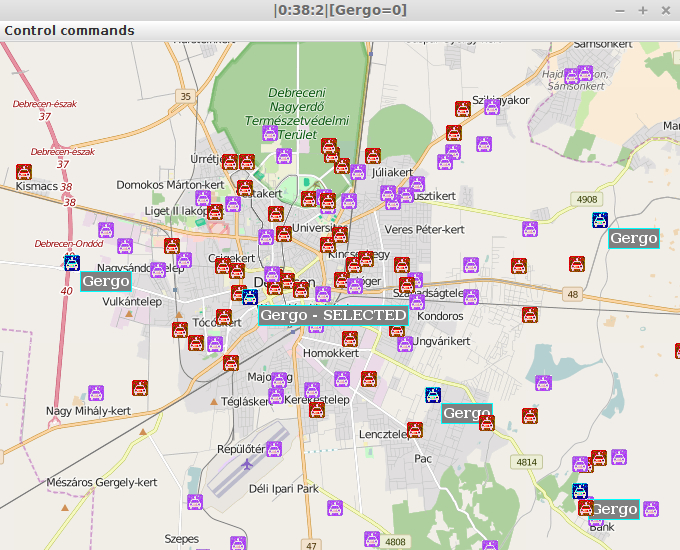
\includegraphics[width=6in]{img/copselected}}
\caption{Pillanatkép a rendszer ``Police Edition'' változatának a projekt szerinti módosításával (lásd: \ref{theapp}. fejezet). A térkép az OSM egy részlete, Debrecen, Hajdú-Bihar Megye, Magyarország. A megjelenítést a JXMapViewer2 \cite{jxmapv} biztosítja. A térképen a routine car rózsaszínnel, a gengszter ágensek pirossal (smart car), a rendőrágensek (guided car) kékkel jelölve. Az éppen kiválasztott rendőr-ágens melyet éppen irányítunk pedig el van látva a ``SELECTED'' felirattal. Forrás: \cite{infocomjournal} 
\label{police}}
\end{figure}

Ennek a projektnek a célja az, hogy az OOCWC (\ref{oocwc}. fejezet) kvalifikációs (illetve a bátrabbaknak a verseny) részét (is) valósidejű irányítás válthassa ki, ezáltal érdekesebbé, és kézügyességtől (is) függővé válik a gengszterek elkapása.

\vspace{2mm}
A projekt egy Maven (\ref{maven}. fejezet) által menedzselt Java (\ref{java}. fejezet) alkalmazás, amihez egy Swing (\ref{swing}. fejezet) grafikus felhasználói felület (Graphic User Interface) tartozik. Továbbá a Maven felelős a projekt dependenciáinak (dependency) a megfelelő verziószámú letöltéséért is. 

\vspace{2mm}
Ilyen függőség például JXMapViewer2 \cite{jxmapv} (\ref{jxmapviewer}. fejezet)).


\section{Az alkalmazás elindítása}
\label{howtorun}

TODO képek importálásról + parancsok

\section{Az alkalmazás funkciói}
\label{functions}


\subsection{Aktuális állás megjelenítése}
\label{actualstate}

Az aktuális állást egyrészt a főképernyőn lehet látni, másrészt az alkalmazás fejlécében összegezve van hogy a szimuláció mennyi időnél tart, illetve hogy melyik rendőrcsapat összesen hány gengsztert kapott el eddig.

TODO

\subsection{Rendőrök és gengszterek hozzáadása}
\label{addcops}

Az alkalmazásban lehetőség van:

\begin{itemize}
\item 1 rendőr hozzáadására (\ref{init1cop}. forráskód);
\item 10 rendőr hozzáadására (\ref{init10cop}. forráskód);
\item 100 gengszter hozzáadására (\ref{init100gangster}. forráskód).
\end{itemize}

\lstinputlisting[language=bash, caption=1 rendőr hozzáadása; ahol a ``Gergo'' a rendőr csapatnevét jelenti., label=init1cop]{src/init_1_cop.sh}

\lstinputlisting[language=bash, caption=10 rendőr hozzáadása; ahol a ``Gergo'' a rendőrök csapatnevét jelenti., label=init10cop]{src/init_10_cop.sh}

\lstinputlisting[language=bash, caption=100 gengszter hozzáadása; ahol a ``Gergo'' azt a csapatnak a nevét jelenti amely hozzáadta a gengsztereket., label=init100gangster]{src/init_100_gangsters.sh}

Mindhárom parancs működösénék az alapelve megegyezik. A telnet protokollt felhasználva elküldjük a kívánt parancsnak megfelelő üzenetet, amit a szimulációs szerver feldolgoz. Ezeknek a parancsoknak az eredményeit azonnal láthatjuk (Erről többet a \ref{dataflow}. fejezetben lehet olvasni).

\vspace{2mm}
Ezeknek a megoldásoknak az előnye hogy a parancsok egy teljesen különböző processzként futnak mint az alkalmazás, ezáltal nem zavarják a folyamatos adatáramlást, ami a megjelenítéshez szükséges. Példa az alkalmazásból 100 gengszter inicializálására a \ref{call100gangster}. forráskódrészletben látható.

\lstinputlisting[language=Java, caption=100 gengszter hozzáadása a \ref{init100gangster}. forráskódot felhasználva Java nyelven., label=call100gangster]{src/call100gangster.java}

\subsection{Rendőrök irányítása}
\label{controlcops}

Miután már van saját rendőrünk a szimulációban (lásd: \ref{addcops}. fejezet), Tudjuk őket irányítani is.

\vspace{2mm}
Alaphelyzetben nincs egy rendőr se kiválasztva. Ahhoz hogy egy rendőr-ágenst irányítani tudjunk egy rendőr közelébe kell kattintanunk a bal egérgombbal, és légvonalban 2500 méteren belül kell lennie a kattintás térképre vetített pontjának a rendőr helyzetétől. Amennyiben már volt kijelölve egy rendőr, de le szeretnénk venni a jelölést, úgy egyszerűen csak egy olyan pontra kell kattintanunk, amely nem esik bele egy rendőr 2,5 kilométeres körébe sem. Ennek a megvalósítása a \ref{selectcop}. forráskódrészleten látható.

lstinputlisting

\newpage
\chapter{Jövőbeli munka}
\label{futureworks}

<TODO szépen leírni>

Mesterséges intelligencia alkalmazása a rendőrök irányítására Java oldalon. 

A program többszálasítása, ahol az egyik szál a megjelenítésért felel, a másik szálon pedig a parancsokat tudnánk küldeni a servernek. Egyelőre nem lehetséges mert 2 egymás mellett futó traffic serverre lenne hozzá szükség, mert jelenleg a 2 szál ugyanarra a socketre bindolna mert ugyanaz a hostname és a port is egy traffic server esetén. 

Spring alapú webszerverré is tovább lehetne fejleszteni, amivel egy webalkalmazássá formálnánk a programot. Ekkor különválik egy backendre (Spring a már meglévő business logic-kal a megjelenítés nélkül) és egy frontendre (AngularJS + Bootstrap | megjelenítés + irányítás). Ez azért lenne érdekes mert egyszerre akár az összes versenyző tudná valós időben irányítani a rendőreit. 

</TODO szépen leírni>

\newpage
\chapter{Összefoglalás}
\label{summary}

TODO

\newpage
\addcontentsline{toc}{chapter}{Irodalomjegyzék}

\begin{singlespace}
\bibliography{copcontroller}
\end{singlespace}

\chapter*{Függelék}
\addcontentsline{toc}{chapter}{Függelék}

\noindent
COPCONTROLLER is free software: you can redistribute it and/or modify
it under the terms of the GNU General Public License as published by
the Free Software Foundation, either version 3 of the License, or
(at your option) any later version.

\noindent
COPCONTROLLER is distributed in the hope that it will be useful,
but WITHOUT ANY WARRANTY; without even the implied warranty of
MERCHANTABILITY or FITNESS FOR A PARTICULAR PURPOSE.  See the
GNU General Public License for more details.

\noindent
You should have received a copy of the GNU General Public License
along with COPCONTROLLER. If not, see <http://www.gnu.org/licenses/>.

\chapter*{Köszönetnyilvánítás}
\addcontentsline{toc}{chapter}{Köszönetnyilvánítás}


\end{document}
